\section{Wstęp}
Przedmiotem projektu jest obiekt opisany w przestrzeni stanów następującym modelem:
\begin{equation}
\frac{dx_{1}(t)}{dt} = -\frac{T_{1}+T_{2}}{T_{1}T_{2}}x_{1}(t) + x_{2}(t)
\end{equation}
\begin{equation}
\frac{dx_{2}(t)}{dt} = -\frac{1}{T_{1}T_{2}}x_{1}(t) + \frac{K}{T_{1}T_{2}}(\alpha_{1}u(t) + \alpha_{2}u^2(t) + \alpha_{3}u^3(t) + \alpha_{4}u^4(t))
\end{equation}
\begin{equation}
y(t)=x_{1}(t)
\end{equation}
gdzie: $$K = 2, T_{1} = 9, T_{2} = 6, \alpha_{1} = 0.15, \alpha_{2} = -0.16, \alpha_{3} = 0.25, \alpha_{4} = 0.43$$ Sygnał sterujący spełnia warunek:
\begin{equation}
-1\leq u \leq 1
\end{equation}
Wszystkie obliczenia, symulacje oraz wykresy wykonane zostały w środowisku Matlab wraz z toolboxem Simulink. Kod służący do wykonywania projektu został zamieszczony w skrypcie $MODIprojekt1.m$, bedącym załącznikiem do poniższego sprawozdania i nie będzie tutaj przytaczany. Poszczególne zadania umieszczone są w osobnych sekcjach, jednak zaleca się conajmniej jednorazowe uruchomienie całego skryptu ze względu na zależności pomiędzy niektórymi punktami projektu. Graficzne reprezentacje poszczególnych modeli wykonane zostały w Simulinku i zawarte są w plikach $zad1.slx$, $zad2.slx$ oraz $zad8.slx$, wywoływanych bezpośrednio z głównego skryptu.
\section{Wykonanie zadań.}
\subsection{Reprezentacja graficzna dynamicznego modelu ciągłego.}
Reprezentacja graficzna dynamicznego modelu ciągłego zawarta została w pliku $zad1.slx$.
\begin{figure}[H]
\centering
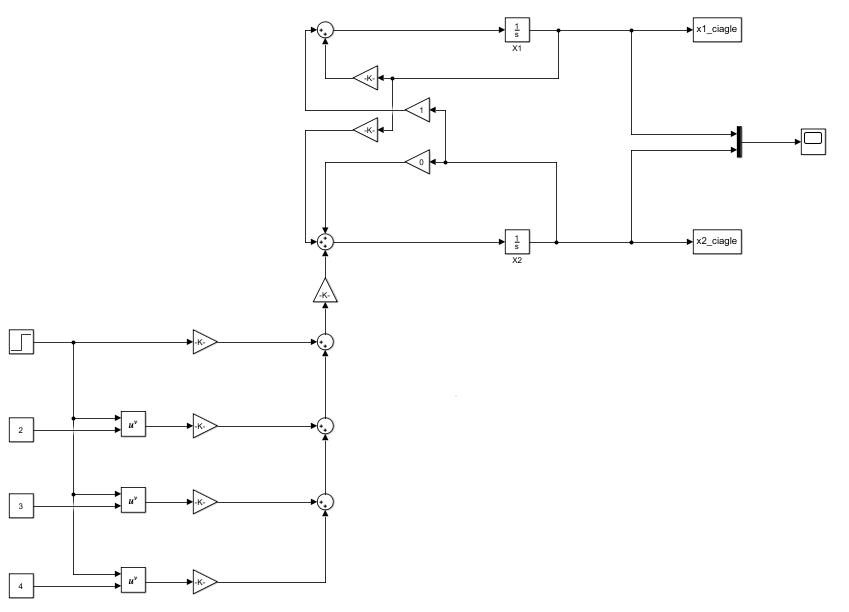
\includegraphics[width=15cm]{images/zad1.png}
\caption{Rozwiązanie zadania 1 - model dynamiczny ciągły}
\label{fig:zad2}
\end{figure}
\subsection{Wyznaczenie oraz reprezentacja graficzna dynamicznego modelu dyskretnego.}
W celu wyznaczenia modelu dyskretnego wykorzystano dyskretyzację metodą Eulera (dokładnie: aproksymację prostokątną w przód), to znaczy:
\begin{equation}
\dot{x}(k) = \frac{x(k+1)-x(k)}{T}
\end{equation}
gdzie: T - okres próbkowania. \\
Podstawiając powyższą zależność do równań 1. oraz 2. otrzymamy model dyskretny w postaci równań różnicowych:
\begin{equation}
x_{1}(k+1)= -\frac{T(T_{1}+T_{2}+1)}{T_{1}T_{2}}x_{1}(k) + Tx_{2}(k)
\end{equation}
\begin{equation}
x_{2}(k+1)= -\frac{T}{T_{1}T_{2}}x_{1}(k) + x_{2}+\frac{KT}{T_{1}T_{2}}(\alpha_{1}u(k) + \alpha_{2}u^2(k) + \alpha_{3}u^3(k) + \alpha_{4}u^4(k))
\end{equation}
\begin{equation}
y(t)=x_{1}(k)
\end{equation}
Reprezentacja graficzna dynamicznego modelu dyskretnego zawarta została w pliku $zad2.slx$.
\begin{figure}[H]
\centering
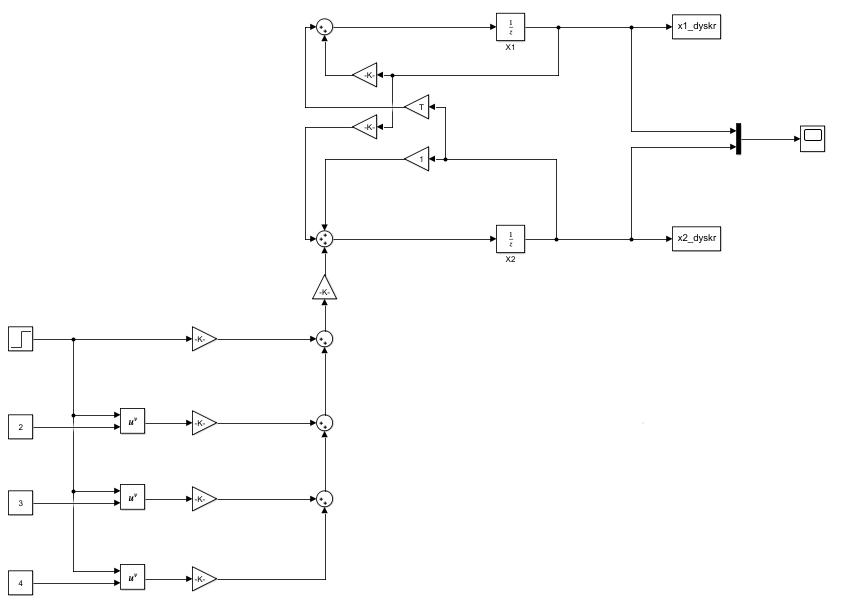
\includegraphics[width=15cm]{images/zad2.png}
\caption{Rozwiązanie zadania 2 - model dynamiczny dyskretny}
\label{fig:zad2}
\end{figure}
\subsection{Porównanie odpowiedzi skokowych modeli ciągłego oraz dyskretnego.}
Sprawdzono układy dyskretne dla różnych wartości okresu próbkowania T.
\begin{figure}[H]
\centering
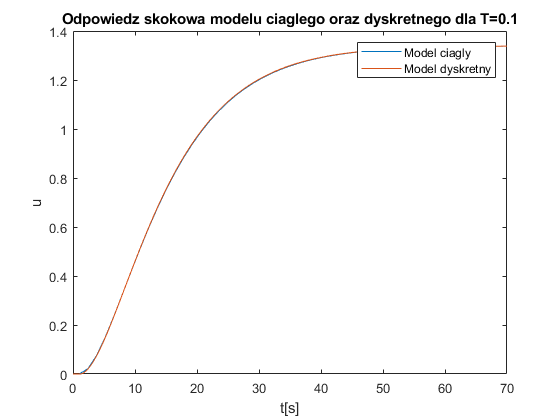
\includegraphics[width=15cm]{images/1.png}
\caption{Rozwiązanie zadania 3 - T=0.1}
\label{fig:1}
\end{figure}
\begin{figure}[H]
\centering
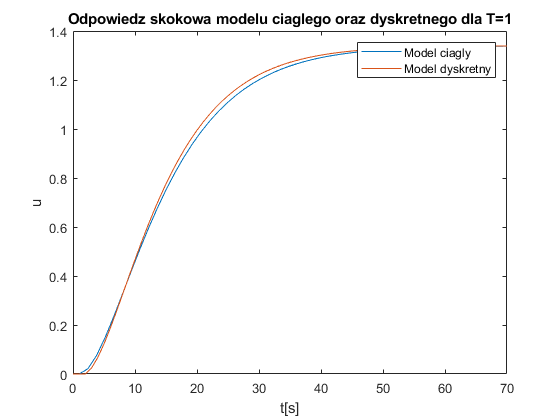
\includegraphics[width=15cm]{images/2.png}
\caption{Rozwiązanie zadania 3 - T=1}
\label{fig:2}
\end{figure}
\begin{figure}[H]
\centering
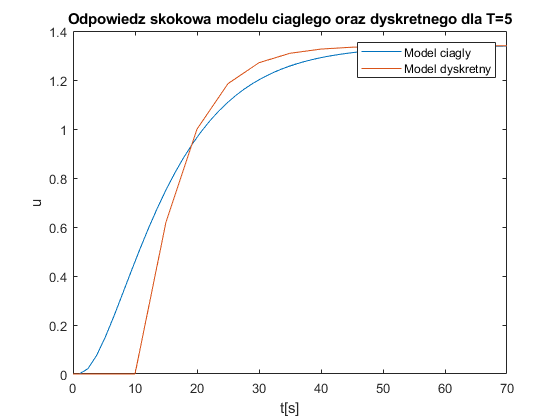
\includegraphics[width=15cm]{images/3.png}
\caption{Rozwiązanie zadania 3 - T=5}
\label{fig:3}
\end{figure}
Jak widać, im większy jest okres próbkowania, tym gorsze jest odwzorowanie dynamiki układu ciągłego przez układ dyskretny. Wartości ustalone jednak są identyczne, co sugeruje, że zgodnie z oczekiwaniem, charakterystyka statyczna modelu dyskretnego nie zależy od okresu próbkowania.
\subsection{Charakterystyka statyczna.}
Charakterystyka statyczna modelu dyskretnego została wyznaczona na dwa dwa sposoby: eksperymentalnie przy użyciu narzedzia Simulink oraz analitycznie - przekształcając równanie dynamiczne.
\subsubsection{Wyznaczenie eksperymentalne.}
Charakterystyka statyczna może zostać wyznaczona eksperymentalnie, poprzez przeprowadzenie szeregu symulacji dla różnych wartości wielkości wejściowe u, a następnie przyjęcie za wartość $y_{stat}(u)$ wartości po ustaleniu wyjścia.
\subsubsection{Wyznaczenie analityczne.}
W stanie ustalonym, przy ustalonym sygnale wejściowym $u$, wartości zmiennych stanu nie zmieniają się, czyli: $\dot{x}(k) = 0$, czyli $x(k)=x(k+1)=x(k+2)=...=x$ Podstawiając te zależności pod równania 6. oraz 7. można wyznaczyć zależności pomiędzy zmiennymi stanu, a ostatecznie - równanie na wartość wyjściową modelu statycznego:
\begin{equation}
y(u)=K \dot (\alpha_{1}u + \alpha_{2}u^2+\alpha_{3}u^3+\alpha_{4}u^4)
\end{equation}
Porówanie otrzymanych charakterystyk statycznych:
\begin{figure}[H]
\centering
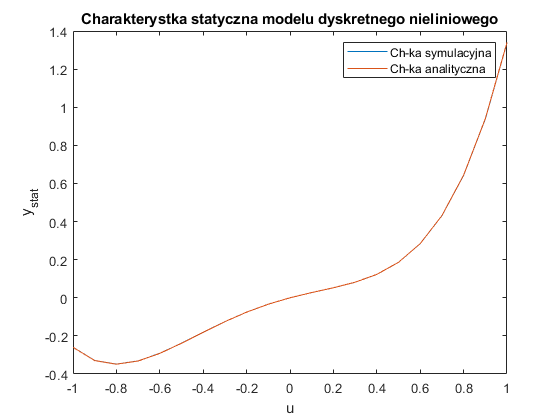
\includegraphics[width=15cm]{images/4.png}
\caption{Rozwiązanie zadania 4}
\label{fig:4}
\end{figure}
\subsection{Charakterystyka statyczna zlinearyzowana.}
Do zlinearyzowania funkcji posłużymy się pierwszymi dwoma wyrazami ciągu Taylora. Zakładamy,
że $\bar{u}$ to punkt linearyzacji.
\begin{equation}
y(u) \approx y(\bar{u}) + \frac{dy(\bar{u})}{du}(u - \bar{u})
\end{equation}
Otrzymano następujący wzór na zlinearyzowaną charakterystykę statyczną w punkcie linearyzacji $\bar{u}$:
\begin{equation}
y(u) = K \dot (4\alpha_{4}\bar{u}^3 + 3\alpha_{3}\bar{u}^2 + 2\alpha_{2}\bar{u} + \alpha_{1})u - K \dot (3\alpha_{4}\bar{u}^4 + 2\alpha_{3}\bar{u}^3 + \alpha_{2}\bar{u}^2)
\end{equation}
\begin{figure}[H]
\centering
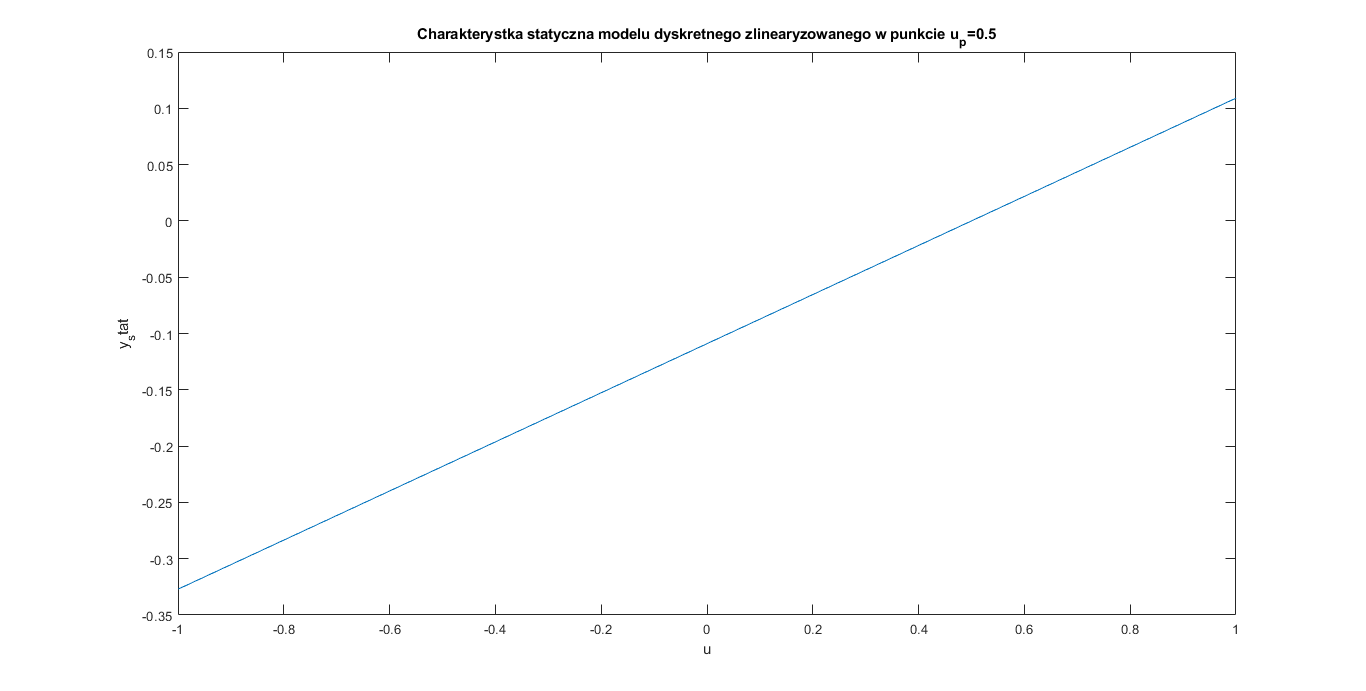
\includegraphics[width=15cm]{images/5.png}
\caption{Rozwiązanie zadania 4 - punkt linearyzacji $\bar{u}=0.5$}
\label{fig:5}
\end{figure}
\subsection{Porównanie charakterystyk statycznej - liniowej oraz nieliniowej.}
Poniżej przedstawiono zlinearyzowane charakterystki statyczne otrzymane dla różnych punktów linearyzacji wraz z charakterystyką statyczną obiektu nieliniowego:
\begin{figure}[H]
\centering
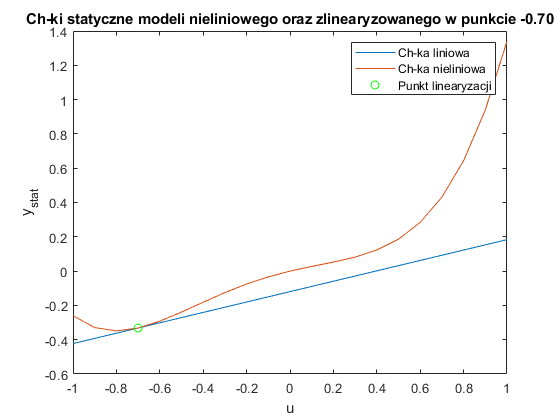
\includegraphics[width=15cm]{images/6.png}
\caption{Rozwiązanie zadania 6 - punkt linearyzacji $\bar{u}=-0.7$}
\label{fig:6}
\end{figure}
\begin{figure}[H]
\centering
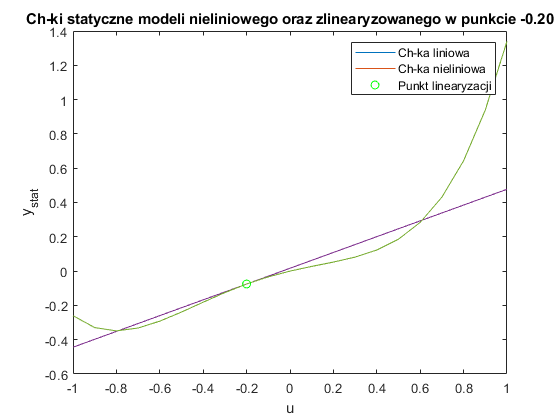
\includegraphics[width=15cm]{images/7.png}
\caption{Rozwiązanie zadania 6 - punkt linearyzacji $\bar{u}=-0.2$}
\label{fig:7}
\end{figure}
\begin{figure}[H]
\centering
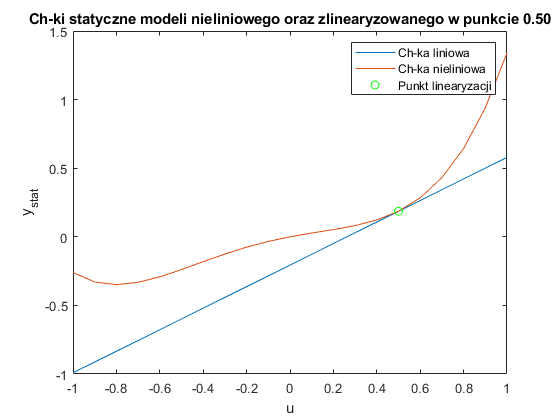
\includegraphics[width=15cm]{images/8.png}
\caption{Rozwiązanie zadania 6 - punkt linearyzacji $\bar{u}=0.5$}
\label{fig:8}
\end{figure}
\begin{figure}[H]
\centering
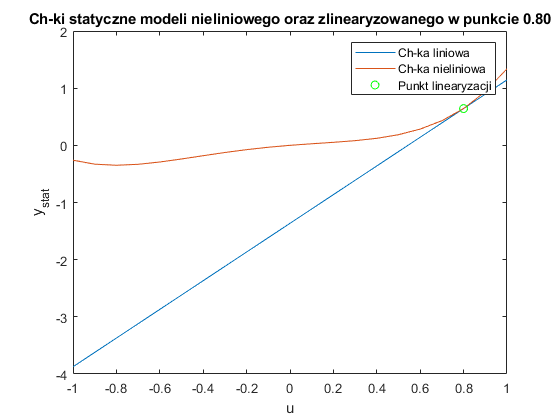
\includegraphics[width=15cm]{images/9.png}
\caption{Rozwiązanie zadania 6 - punkt linearyzacji $\bar{u}=0.8$}
\label{fig:9}
\end{figure}
\subsection{Zlinearyzowany model dynamiczny dyskretny.}
Tą samą metodą co charakterystykę statyczną, można dokonać linearyzacji modelu dyskretnego. Linearyzacja będzie występować wyłącznie w równaniu 7. \\
Zlinearyzowany model dyskretny w postaci równań stanu:
\begin{equation}
\frac{dx_{1}(t)}{dt} = -\frac{T_{1}+T_{2}}{T_{1}T_{2}}x_{1}(t) + x_{2}(t)
\end{equation}
\begin{multline}
\frac{dx_{2}(t)}{dt} = -\frac{1}{T_{1}T_{2}}x_{1}(t) + \frac{K}{T_{1}T_{2}}(\alpha_{1}(\bar{u}+(u(t)-\bar{u})) + \alpha_{2}(\bar{u}^2 + 2\bar{u}(u(t)-\bar{u})) \\
+\alpha_{3}(\bar{u}^3 + 3(\bar{u}^2)(u(t)-\bar{u}))+\alpha_{4}  (\bar{u}^4 + 4(\alpha{u}^3)(u(t)-\bar{u})))
\end{multline}
\begin{equation}
y(t)=x_{1}(t)
\end{equation}
\subsection{Reprezentacja graficzna zlinearyzowanego dynamicznego modelu dyskretnego.}
Reprezentacja graficzna zlinearyzowanego dynamicznego modelu dyskretnego zawarta została w pliku $zad8.slx$.
\begin{figure}[H]
\centering
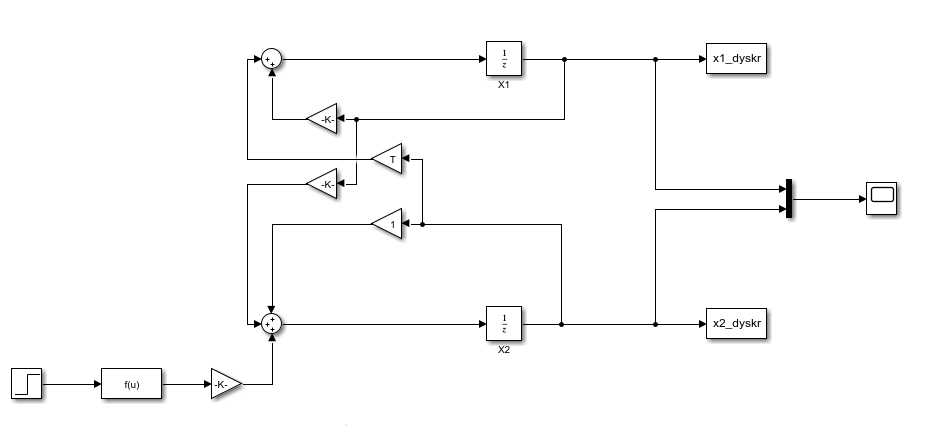
\includegraphics[width=15cm]{images/zad8.png}
\caption{Rozwiązanie zadania 8}
\label{fig:zad8}
\end{figure}
W celu uproszczenia zapisu, część równania dotycząca sygnału wejściowego, została przedstawiona w formie bloku funkcyjnego. Zawiera on równanie:
\begin{multline}
f(u) = \frac{K}{T_{1}T_{2}}(\alpha_{1}(\bar{u}+(u(t)-\bar{u})) + \alpha_{2}(\bar{u}^2 + 2\bar{u}(u(t)-\bar{u})) \\
+\alpha_{3}(\bar{u}^3 + 3(\bar{u}^2)(u(t)-\bar{u}))+\alpha_{4}  (\bar{u}^4 + 4(\alpha{u}^3)(u(t)-\bar{u})))
\end{multline}
\subsection{Porównanie odpowiedzi skokowych modeli dyskretnych - nieliniowego oraz zlinearyzowanego.}
Poniżej przedstawiono odpowiedzi modeli dyskretnych, nieliniowego oraz zlineryzowanego, na skoki wielkości wejściowej $u$ (o różnych wartościach) z punktu pracy, dla którego został wyznaczony model zlinearyzowany. Skoki wykonywano o wartości $\Delta u=0.05,0.1,0.15$.
\begin{figure}[H]
\centering
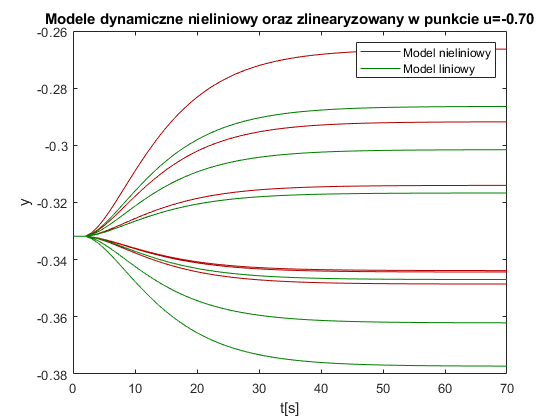
\includegraphics[width=15cm]{images/10.png}
\caption{Rozwiązanie zadania 9}
\label{fig:10}
\end{figure}
\begin{figure}[H]
\centering
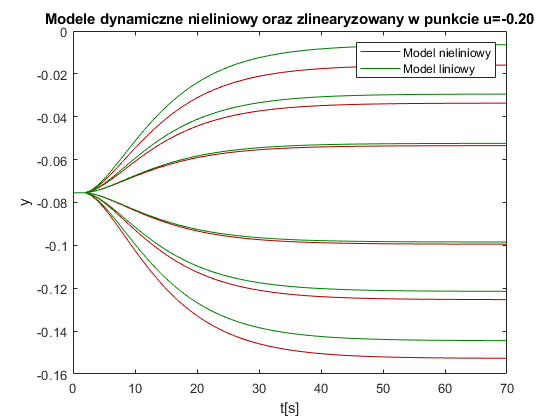
\includegraphics[width=15cm]{images/11.png}
\caption{Rozwiązanie zadania 9}
\label{fig:11}
\end{figure}
\begin{figure}[H]
\centering
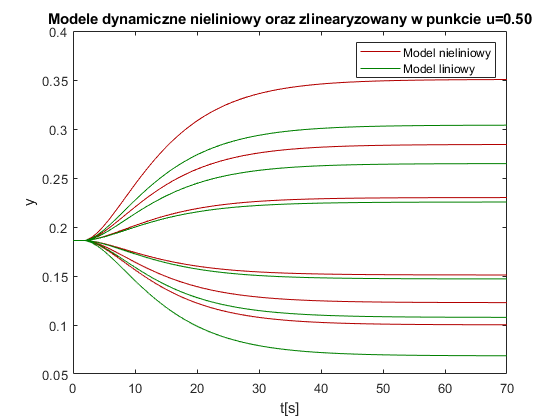
\includegraphics[width=15cm]{images/12.png}
\caption{Rozwiązanie zadania 9}
\label{fig:12}
\end{figure}
\begin{figure}[H]
\centering
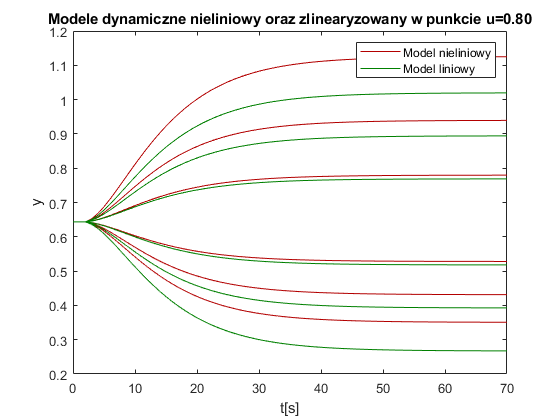
\includegraphics[width=15cm]{images/13.png}
\caption{Rozwiązanie zadania 9}
\label{fig:13}
\end{figure}
\subsection{Model w postaci transmitancji dyskretnej.}
W celu wyznaczenia modelu w postaci transmitancji dyskretnej, usuniemy wyrazy stałe z utworzonego wcześniej model zlinearyzowanego. Otrzymamy w ten sposób model w postaci:
\begin{equation}
\frac{dx(t)}{dt} = Ax(t) + Bu(t)
\end{equation}
\begin{equation}
y(t)=Cx(t) + Du(t)
\end{equation}
W ten sposób wyznaczono poszczególne macierze modelu: \\
\begin{multline}
A=
\begin{bmatrix}
    (1-T\frac{T_{1}+T_{2}}{T_{1}+T_{2}}) & T \\
    \frac{-T}{T_{1}T_{2}} & 1
\end{bmatrix}
B=
\begin{bmatrix}
    0 \\
    \frac{KT}{T_{1}T_{2}} \dot (\alpha_{1} + 2\alpha_{2}\bar{u} + 3\alpha_{3}\bar{u}^2 + 4\alpha_{4}\bar{u}^3)
\end{bmatrix}
C=
\begin{bmatrix}
    1 & 0 \\
\end{bmatrix}
D=
\begin{bmatrix}
     0
\end{bmatrix}
\end{multline}
Następnie korzystając z poniższego równania wyznaczono transmitancję:
\begin{equation}
G(z)=C(Iz-A)^{-1}B + D
\end{equation}
\begin{equation}
G(z)=
\frac{4K\alpha_{4}T^2\bar{u}^3 + 3K\alpha_{3}T^2\bar{u}^2 + 2K\alpha_{2}T^2\bar{u} + K\alpha_{1}T^2}{T_{1}T_{2}z^2 + (TT_{1} + TT_{2} - 2T_{1}T_{2})z + T_{1}T_{2} - TT_{2} - TT_{1} + T^2}
\end{equation}
Transmitancja modeli zlinearyzowanych wyznaczonych dla wcześniej używanych punktów linearyzacji:
\begin{equation}
G(z)\bigg\rvert_{\bar{u}=-0.7}=\frac{174713724808121727}{31128880624384868352z^2 - 53610849964218384384z + 23058430092136939520}
\end{equation}
\begin{equation}
G(z)\bigg\rvert_{\bar{u}=-0.2}=\frac{33181080902585055}{3891110078048108544z^2 - 6701356245527298048z + 2882303761517117440}
\end{equation}
\begin{equation}
G(z)\bigg\rvert_{\bar{u}=0.5}=\frac{157}{10800z^2 - 18600z + 8000}
\end{equation}
\begin{equation}
G(z)\bigg\rvert_{\bar{u}=0.8}=\frac{180812679567491835}{3891110078048108544z^2 - 6701356245527298048z + 2882303761517117440}
\end{equation}
\subsection{Zależność wzmocnienia statycznego od punktu pracy.}
Z definicji, wzmocnienie statyczne transmitancji można wyznaczyć obliczając granicę z transmitancji dla z dażącego do jedności:
\begin{equation}
K_{stat}=lim_{z=1}G(z) = 4K\alpha_{4}\bar{u}^3 + 3K\alpha_{3}\bar{u}^2 + 2K\alpha_{2}\bar{u} + K\alpha_{1}
\end{equation}
Poniżej przedstawiono charakterystykę, która przedstawia zależność wzmocnienia statycznego od danego punktu pracy.
\begin{figure}[H]
\centering
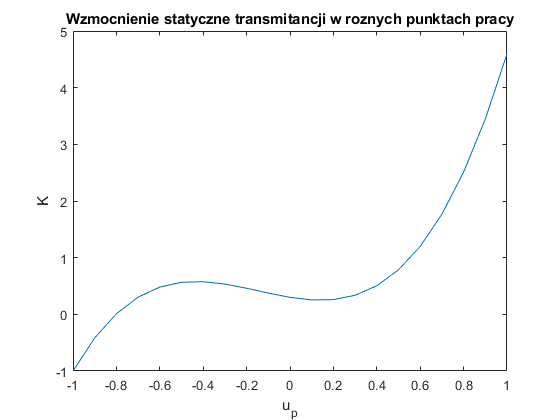
\includegraphics[width=15cm]{images/14.png}
\caption{Rozwiązanie zadania 11 - charakterystyka $K_{stat}(u)$}
\label{fig:14}
\end{figure}
\subsection{Porównanie wzmocnienia statycznego transmitancji oraz modelu zlinearyzowanego.}
Aby wyznaczyć wzmocnienie statyczne modelu zlinearyzowanego należy:
\begin{enumerate}
\item Wykonać skok o dowolną wartość i zmierzyć wartość wyjściową po ustaleniu przebiegu (wartość statyczna),
\item Wykonać kolejny skok o ustaloną wartość, większą o $\Delta u$, a następnie ponownie odczytać wartość wyjściową po ustaleniu przebiegu,
\item Wartość wzmocnienia statycznego otrzymamy poprzez odjęcie kolejnej wartości statycznej od poprzedniej, a następnie podzieleniu przez przyrost skoku $\Delta u$.
\end{enumerate}
\begin{equation}
K_{stat}(\bar{u})=\frac{y_{stat}(\bar{u}+\Delta u) - y_{stat}(\bar{u})}{\Delta u}
\end{equation}
Otrzymane w ten sposób wartości wzmocnienia statycznego porównano z wartościami wzmocnienia statycznego obliczonego przy użyciu transmitancji z kolejnych punktów pracy: -0.7, -0.2, 0.5.
\begin{figure}[H]
\centering
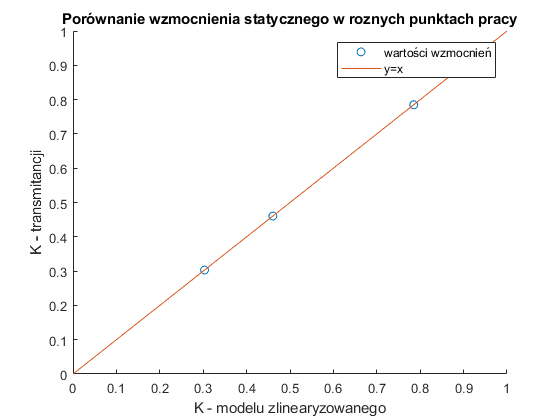
\includegraphics[width=15cm]{images/15.png}
\caption{Rozwiązanie zadania dodatkowego - porównanie wzmocnień statycznych}
\label{fig:15}
\end{figure}
\section{Wnioski}
\begin{itemize}
\item Zgodnie z oczekiwaniami, odpowiedzi skokowe modeli zlinearyzowanych są symetryczne dla przeciwnych wartości skoków, a im większa jego amplituda,  tym większa różnica między odpowiedzią skokową modeli zlinearyzowanych a modelu nieliniowego.
\item Wartości wzmocnienia statycznego uzyskanego poprzez symulacje modeli zlinearyzowanych oraz przy użyciu transmitancji są identyczne,
\item Transmitancje dyskretne często mają skomplikowaną strukturę ze względu na występujące w niej niecałkowite wartości liczbowe. Z tego względu, funkcja programu Matlab $\textit{collect}$, wymuszająca użycie liczb całkowitych, zwraca kilkudziesięcocyfrowe wartości (będące najmniejszymi wspólnymi wielokrotności)
\end{itemize}